% Chapter 2

\chapter{Methodology and approach} % Write in your own chapter title
\label{Chapter2}

\section{Image analysis tools}

\indent Matlab and OpenCV ~\cite{34} are two highly used image
processing tools.  Matlab comes with rich image processing and analysis
libraries. It supports most of the work discussed in introduction
chapter. Matlab also provides interface to convert the code into a C
code. However, generated C code is normally very bulky and takes higher
execution time. OpenCV is an open source computer vision library
initiated by intel. It is available at
http://SourceForge.net/projects/opencvlibrary. It can be used for
research or even commercial purposes. Unlike GNU Public License (GPL),
it's licensing does not force that modifications to the library be made
public. \\

\indent OpenCV has been mainly developed in C and C++ on Linux platform.
However, interfaces for other scripting language such as Python, Ruby
etc are also being developed. OpenCV libraries have been used in many
applications since its first release in 1999.\\

\indent OpenCV design goal is to build computer vision library with
computational efficiency which can work with real time applications. It
contains functions in almost all the area of image processing  and
computer vision like, histogram processing, morphological processing,
segmentation, detection tracking, camera calibration etc. Therefore,
selection of OpenCV libraries allows faster evaluation and development
of real embedded application.\\

\indent OpenCV libraries are also available for embedded architecture
CPUs like ARM. This allows easy porting of applications developed on x86
platform to ARM or other embedded platforms.\\

\indent Therefore, we decided to implement our image pipeline in C and
on Linux platform, so that it can easily be ported from a PC to embedded
environment. Wherever possible, we have used OpenCV library to carry
intended job.


\section{Image Pipeline}


\indent Top level surveillance pipeline can be thought of as in figure
~\ref{image_pipeline}.  End goal of low bandwidth pipeline would be to
generate information such as human detected, their position and the time
of detection. So, to implement above pipeline we have to decide on
following items, computational efficiency and true detection for
considered object has to be kept as primary objective while making any
decision.

\begin{figure}[!t]
\centering
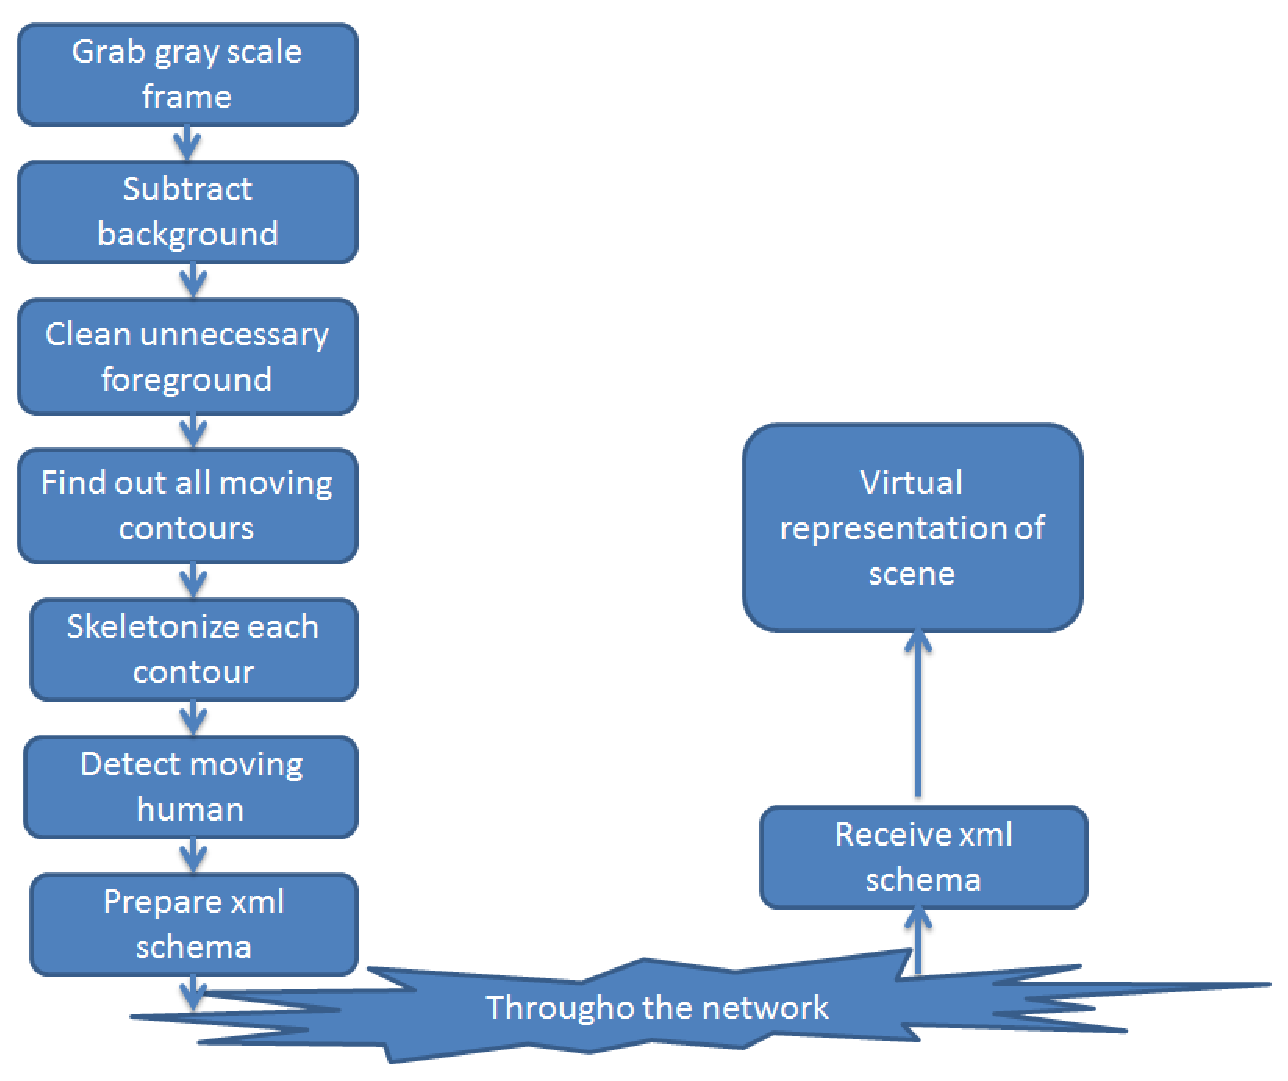
\includegraphics[height=300pt]{Figures/image_pipeline}
\caption{Low bandwidth surveillance Image Pipeline}
\label{image_pipeline}
\end{figure}

\begin{enumerate}

 \item  \textbf{Background Subtraction:} Methods based on LBP by Yao and
Odobez ~\cite{11} have striking nice result. It works superbly with
varied background situation like wavering tree, moving escalator etc.
Barnich and Van Droogenbroeck claims that Vibe which uses random sample
selection also performs well in all situation and have extremely low
computational cost. Yao and Odobez have provided their C code, however
Barnich and Van Droogenbroeck have only provided an object library for
x86 platform. Therefore we need to first code vibe in C and then to
compare above two algorithms.

\item \textbf{Detection and Tracking:} Method based on skeleton motion
features ~\cite{32, 22, 31} seems to be computationally efficient. So we
need to evaluate different method of skeletonization, suitable for
motion calculation. Performance of detector based on such method need to
be compared with other methods based on covariance feature with cascade
of logitboost classifier ~\cite{19}  and Haar like features ~\cite{17}
for which C codes are already available in public domain.
 
\item \textbf{Embedded implementation:} It is very important to see
performance of pipeline based on different algorithm on real embedded
platform. ARM controller is used in most of the embedded multimedia
applications. So, it will be nice to observe their performance with ARM
controller.

\end{enumerate}


\section {Evaluation of different techniques for pipeline stages}

\subsection{Frame acquisition}

\indent OpenCV provides a way to grab frames either from a camera or
from a file. cvCaptureFromFile or cvCaptureFromCAM returns CvCapture *
struct which can further be used to query frame from either a test video
file or from camera respectively. cvQueryFrame function reads one frame
and returns its pointer. If camera's output or test video is in RGB mode
then, it need to be converted into gray scale image for further
processing. cvCvtColor function has been used to convert image from RGB
to gray scale.


\subsection{Background removal}

\indent Since background subtraction has key role in accomplishing
intended job, therefore we have compared two recently developed
efficient background subtraction algorithm and then selected one of them
in our final work.  Yao and Odobez ~\cite{11} used texture features
present in Local Binary Pattern(LBP). LBP works well with local
illumination changes, however there can be issues in case of global
illumination change. They have done several improvements by using
photometric invariant color measurement and flexible weight updating for
background modes. However, our experiments says that, computationally it
is very less efficient compared to method proposed by Barnich and Van
Droogenbroeck  ~\cite{9}.  It is based on unique way of replacing
background pixel value over the time. It replaces background values for
last N frames randomly.  Furthermore, it diffuses updated values to
neighbouring pixels, and again that too on random basis. We have
selected method by Barnich and Van Droogenbroeck  in our final pipeline,
because of it's computational efficiency while maintaining quality.
Figure \ref{bg_compare} shows the comparison of execution time of these
two algorithm.

\begin{figure}[!t]
\centering
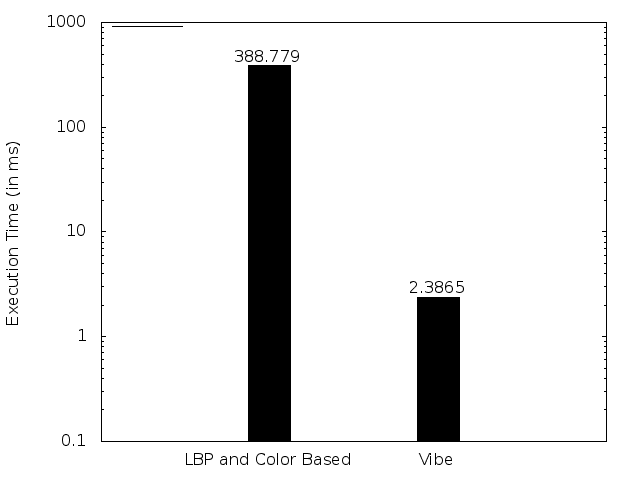
\includegraphics[height=300pt]{Figures/bg_compare}
\caption{Variation of background subtraction execution time of ~\cite{11}
and ~\cite{9} with frame number. This timing was observed with a system
having having DMIPS = 800.}
\label{bg_compare}
\end{figure}

\subsection{Noise removal}

\indent None of the background subtraction algorithm allows pure
foreground extraction. There would always be several noise object in the
extracted image. These are cleaned by morphological erosion operation
(cvErode) followed by dilation (cvDilate) operation. Further all moving
contours are separated out by using OpenCV library function
cvFindContours. This function provides us boundary point of individual
moving object.

\subsection{Skeletonization techniques}

\indent Image skeletons are nice way to represent shape of an object.
This method can be used to identify type of object. We have evaluated
different skeletonization techniques, with their merits and demerits for
suitability to our requirement.\\

\begin{enumerate}
\item \textbf{Contour skeleton:} It is obtained by finding outer
boundary points of an object. It gives idea about global shape of an
object. Boundary points obtained by function cvFindContours can further
be converted into polygon by cvApproxPoly. Vertices of this polygon
connected together gives an idea about outer shape of the object. An
example of such skeleton has been shown in figure
\ref{contour_skeleton}.

\begin{figure}[!t]
\centering

\includegraphics[height=300pt]{Figures/contour_skeleton}
\caption{An example of contour skeleton}
\label{contour_skeleton}
\end{figure}

\item \textbf{Morphological skeleton:} Gonzalez and Woods has provided
a set of morphological operations in his book Digital image processing
~\cite{35}. He has defined morphological skeletonization as follows:

	\begin{eqnarray}
	S(A) = \Sigma ^K _{k = 0} S_k(A) \nonumber \label{morph_skel}\\
		where S_k(A) = (A \ominus kB) - (A \ominus kB)
\circ B \nonumber\\
		k = max \{ K | (A \ominus kB) \neq \phi\}
	\end{eqnarray}

Translating equation ~\ref{morph_skel} into C code:

\begin{lstlisting}

	do
	{
		cvErode(img, eroded, element, 1);
		cvDilate(eroded, temp, element, 1);
		cvSub(img, temp, temp, NULL);
		cvOr(skel, temp, skel, NULL);
		cvCopy(eroded, img);
		done = (cvCountNonZero(img) == 0);
	} while (!done);

\end{lstlisting}

An example of skeleton obtained by morphological method has been
shown in figure \ref{morphological_skeleton}.

\begin{figure}[!t]
\centering
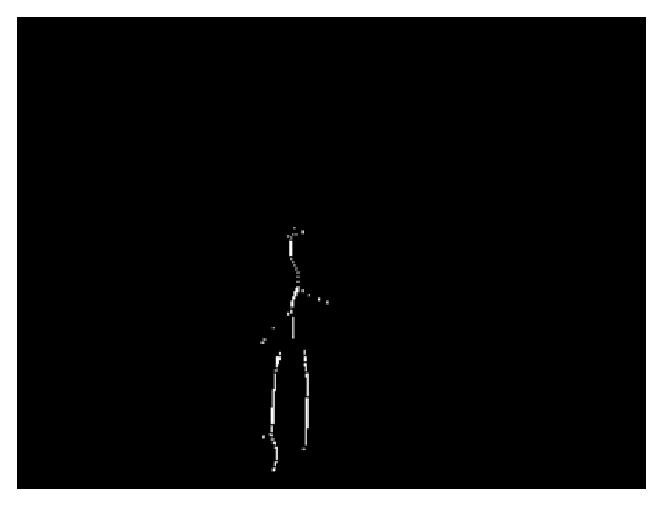
\includegraphics[height=300pt]{Figures/morphological_skeleton}
\caption{An example of morphological skeleton}
\label{morphological_skeleton}
\end{figure}

\item \textbf{Skeleton by distance transform:} Distance transform of an
input image is obtained by creating a new image where pixels are set to
a value equal to the distance to the nearest zero value pixel in input
image. We had seen that contour skeleton provided outer shape of the
object, where as distance transform method provides internal orientation
of object. OpenCV provides a function cvDistTransform, which can be used
to build a distance transformed image. An example of skeleton obtained
by distance transform method has been shown in figure \ref{dt_skeleton}.

\begin{figure}[!t]
\centering
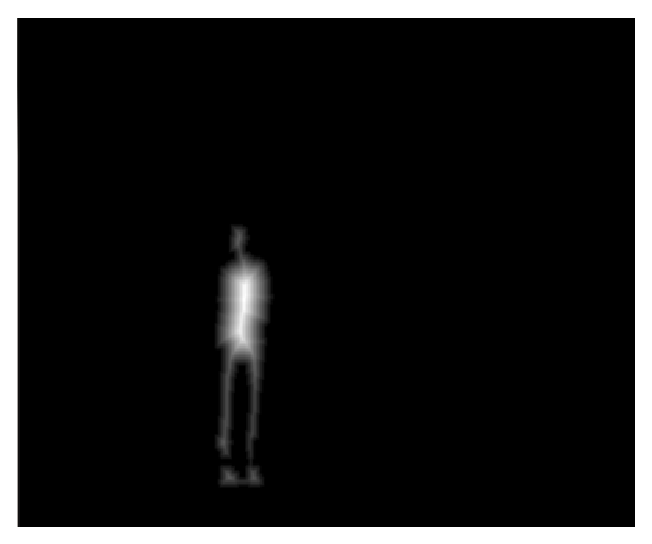
\includegraphics[height=300pt]{Figures/dt_skeleton}
\caption{An example of skeleton obtained by distance transform}
\label{dt_skeleton}
\end{figure}

\item \textbf{Star Skeleton:} In this method we plot distance of each
boundary point from the centroid and then uses peaks of the curve as
skeleton point.
\begin{enumerate}
\item Centroid of each object is found out using following equation
~\ref{centroid_calc}.\\
	\begin{eqnarray}
	C_x = {1 \over N} \Sigma ^N _{i = 1} X_i \label{centroid_calc}
\nonumber \\
	C_y = {1 \over N} \Sigma ^N _{i = 1} Y_i 
	\end{eqnarray}
Here X$_i$ and Y$_i$ are (X,Y) co-ordinate of i$_{th}$ point on the contour
boundary.
\item Distance d$_i$ is calculated between centroid and each boundary
point as follows.This calculated distance vector are stored in a CvMat
array.
	\begin{equation}
	d_i = \sqrt{(C_x - X_i)^2 + (C_y - Y_i)^2} \label{dist_calc}
	\end{equation}

\begin{figure}[!t]
\centering
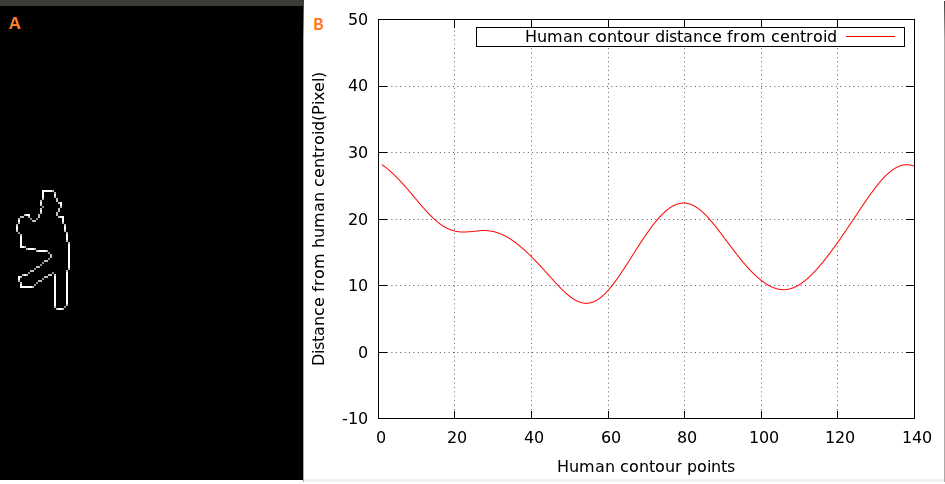
\includegraphics[height=200pt]{Figures/distance}
\caption{Distance plot of human contour points from its centroid}
\label{distance}
\end{figure}

\item Distance vector array is smoothed to remove noise peaks using
cvSmooth. If these distances are plotted then it looks like figure
\ref{distance}. Now local maxima of distance vector is
calculated by finding zero crossing of difference vectors. These local
maxima provides a star form of skeleton centered at centroid of the
object. A typical star skeleton has been shown in figure
~\ref{star_skeleton}.

\begin{figure}[!t]
\centering
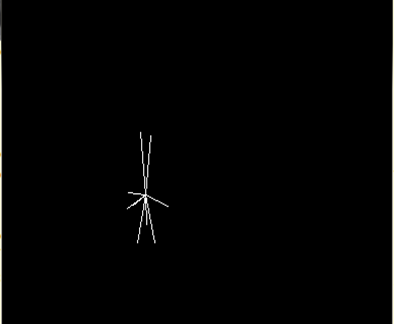
\includegraphics[height=300pt]{Figures/star_skeleton}
\caption{An example of star skeleton}
\label{star_skeleton}
\end{figure}

\end{enumerate}

\end{enumerate}

\subsection{Human detection methods}

We have evaluated three methods of human detection technique mainly on the
basis of their computation efficiency.
\begin{enumerate}
\item \textbf{Detection using covariance features:} We have used method
implemented by Yao and Odobez ~\cite{19}. We have selected this method,
because it has been widely referenced and also C code by author is
available in public domain.\\
\item \textbf{Detection using haar features:} We have evaluated work by
Viola and Jones in ~\cite{16, 17} which uses haar like features for
human detection. Again, reason to evaluate this algorithm was same, that
it has been widely discussed and referenced. It's implementation has
been done in one of the demo example code of OpenCV.\\
\item \textbf{Detection using skeleton motion features:} We have
evaluated this method as it seems to be computationally very efficient.
We have provided C code for our complete pipeline in apendix
~\ref{ApendixA}.  Human motion can be represented suitably by movement
of legs. So, we use star skeletonization method which seems best
suitable for human leg motion analysis. We have seen that star
skeletonization gives us some peaks which is not of our interest. In our
algorithm, we are using 2 most relevant peaks which are nearest to each
bottom corner of bounding box of contour respectively. Only these two
peaks along with centroid will give us sufficient information to
distinguish human among human, vehicle or animal etc.\\
\indent When the case considered is human, then the two peaks correspond to
the two legs of human. When case considered is vehicle, then the peaks
correspond to the two extrema points of lower portion of back and front.
When it is an animal, then peaks correspond to front and back leg of
animal.\\
\indent Let P$_1$(X$_1$, Y$_1$), P$_2$(X$_2$, Y$_2$) and C(C$_x$, C$_y$)
are two peaks nearest to bottom right and bottom left corner and
centroid respectively. Let $\theta$ is the angle between P$_1$C and
P$_2$C, then $\theta$ can be calculated as follows.\\
%
	\begin{equation}
	\theta = tan^{-1}[(Y_2 - C_y) / (X_2 - C_x)] \\ - tan^{-1}[(Y_1 - C_y) / (X_1 - C_x)]
	\end{equation}
%
\indent If variation of this $\theta$ is plotted in respective frames
for human and vehicle then the resultant plot is as shown in fig
\ref{angle_plot}. The observations from this plot is that for human,
angle variation pattern is repeatable, and it is zero for almost at
regular intervals. For vehicle, it is constant. The experiment with
images containing animal is to be carried out. For images with animal in
it, there would be variation with repeatable pattern but would never
touch to zero. These criterion can be the basis to identify about an
object, whether it is a human, vehicle or animal.

\begin{figure}[!b]
\centering
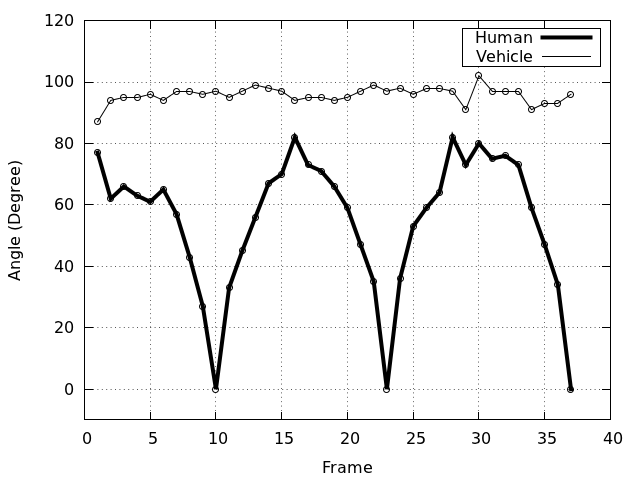
\includegraphics[height=300pt]{Figures/angle_plot}
\caption{Variation of angle between legs with frame number for human and
vehicle.}
\label{angle_plot}
\end{figure}

\indent We create a linked list of objects. When a new object comes in
the view of camera, a structure is created and added to the list. This
new object is tracked and value of (C$_x$, C$_y$), $\theta$ in each
frame is stored.
\begin{enumerate} 
\item We track value of $\theta$ until it goes to zero three times.
\item Now consider $\theta$ values between first and second zero as
vector T$_1$ and $\theta$ values between second and third zero as vector
T$_2$.
\item Find mean m$_1$ and m$_2$ of vector T$_1$ and T$_2$ respectively.
\item If n is the length of vector T$_1$ then calculate correlation value
between these two vectors to find similarities as follows.
	\begin{equation}
	corel = {{\Sigma ^n _{i = 1}(T_{1i} - m_1) * (T_{2i} - m_2)}
\over {\sqrt {\Sigma ^n _{i = 1} (T_{1i} - m_1)^2 * \Sigma ^n _{i = 1} (T_{2i}
- m_2)^2}}}
	\end{equation}
\item If correlation value is greater than a threshold value TH$_1$, then we say
that it is a human.
\end{enumerate} 

\end{enumerate} 


\section {Platforms used for evaluation}

\indent We have developed all our code and used other code taken from
public domain at a x86 based platform (A Linux virtual box on HP
EliteBook 8440P). We have coded in C and on Linux platform. We did it so
because, C and Linux are widely used with embedded platform. Since
latest Linux version such as 3.0 onwards works well with mmuless
platforms too, so it would be very easy to use same code across wide
range of micro-controllers and SOCs.

\indent It is also very important to benchmark the system which we are
using for test evaluation. However, none of the benchmark code provides
accurate figure for interpolation of results for any test, but still
they can be considered as approximate reference. We benchmarked our x86
system with dhrystone code.

\indent We have further evaluated performance of different pipeline on
an ARM11 based system. We have used Raspberry Pi , which has a Broadcom
BCM2835 system on a chip (SoC), that includes an ARM1176JZF-S 700 MHz
processor. We have also benchmarked this system with dhrystone code.
